%
%   TEMPLATE
%   コピペ用
%

\documentclass[10pt,b5paper,papersize,dvipdfmx]{jsbook}

\usepackage{vuccaken}
\usepackage{vuccaken2019}

% スタイルファイルの読み込みや自作マクロは、
% 最終的には vuccaken2019.sty の中に書いてください。
% とりあえずはここに書いてもらって構いません。


\begin{document} % 以下本文

% - - - - - - - - - - - - - - - - - - - - - - - - %
\kaishititle%
  {\LaTeX テンプレート(会誌原稿用)}% title
  {テンプレ科学科4回生}% 所属
  {テンプレくん}% name
% - - - - - - - - - - - - - - - - - - - - - - - - %

% \setcounter{tocdepth}{2} % 目次にどこまで表示するか
% \tableofcontents % 目次出力
% \clearpage % 改ページ

%
\section*{はじめに}
会誌ではjsbookクラスを使います。\par
テーマが複数ある場合は別ファイルで提出してください。

%
\section{セクション}
はじめにこのファイルのソースを自分のtexファイルにコピペしてください。\par
figureのパスには注意してください。

% \begin{figure}[htbp]
%   \centering
%   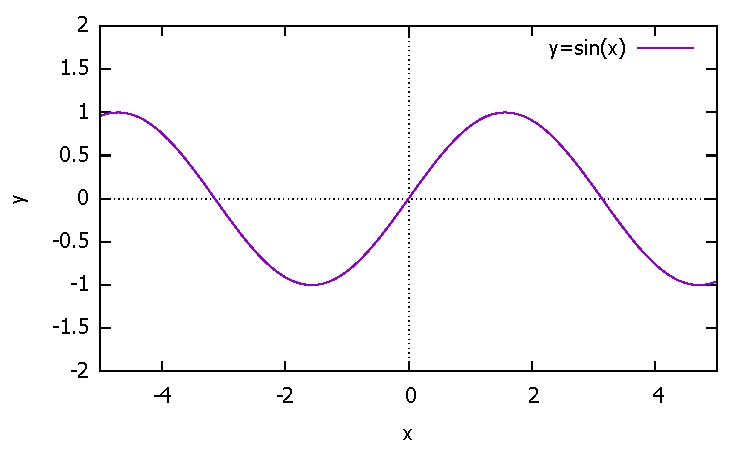
\includegraphics[width=10cm]{temp/fig-sin.pdf}
%   \caption{$y=\sin x$のグラフ。gnuplotで作成した。}
%   \label{fig:sin}
% \end{figure}

%% 参考文献
\begin{sanko}
  \begin{enumerate}
    \item 著者, 本やページの名前, (URL), 出版社, 出版年.
    \item (複数ある場合は追加)
    \item @vuccaken, 物科研HP, \url{rp2017xy.starfree.jp}, 2019.
  \end{enumerate}
\end{sanko}


\end{document}
%
% ファイトだよ!
%
